% Melhorar figuras SVG
% Corrigir referência sub
% Esse caracter: —

\section{Introduction}

Asthma is a chronic inflammatory disease of the airways, characterized by variable airflow obstruction, bronchial hyperresponsiveness, and persistent inflammation. These features are driven by the activation of immune cells — particularly eosinophils, Th2 lymphocytes, and airway epithelial cells — which promote the release of cytokines such as IL-4, IL-5, and IL-13 % [Hamid et al. 2003]
\cite{hamid_inflammatory_2003}. According to the World Health Organization, asthma affected approximately 262 million individuals worldwide in 2019, representing a major global health burden % [Vos et al. 2020]
\cite{vos_2020}. Multiple environmental and socioeconomic factors — including urbanization, exposure to aeroallergens, air pollution, respiratory infections, and health disparities — have contributed to the increasing prevalence and severity of asthma worldwide % [Ni et al. 2024; Zheng et al. 2018; Goldin et al. 2025; Checkley 2019; Chatkin et al. 2022].
\cite{ni_long-term_2024,zheng_regional_2018,goldin_asthma_2025,checkley_what_2019,chatkin_external_2022}.

However, the lack of validated molecular biomarkers for clinical use hinders the accurate stratification of asthma endotypes, hindering the implementation of precision medicine-based therapeutic strategies % [Skloot 2016; Cremades-Jimeno et al. 2021]
\cite{skloot_asthma_2016,cremades-jimeno_prioritizing_2021}. Identifying these biomarkers is crucial for advancing personalized disease management and developing more effective targeted therapies. Studies in the literature have investigated various biomarkers associated with immune cell activation, airway remodeling, and inflammatory pathways. For example, IL-5, periostin, fractional exhaled nitric oxide (FeNO), blood eosinophil count, and serum IgE have been widely evaluated as indicators of inflammations predominant in many asthma phenotypes % [Dweik et al. 2011; Price et al. 2015]
\cite{dweik_official_2011,price_blood_2015}.

Transcriptomic analyses have played a crucial role in biomarker discovery. The study by % [Modena et al. 2017]
\cite{modena_gene_2017} identified transcriptomic signatures associated with severe asthma from bronchial epithelial cells, revealing gene expression profiles linked to corticosteroid resistance and exacerbated inflammation. Similarly, % [Bigler et al. 2017]
\cite{bigler_severe_2017} analyzed gene expression in sputum and reported that high levels of IL1RL1 and CLCA1 were associated with high Th2 endotypes. Furthermore, % [Cremades-Jimeno et al. 2021]
\cite{cremades-jimeno_prioritizing_2021} highlighted the usefulness of multi-omics integration, combining transcriptomics, proteomics, and metabolomics, to refine biomarker selection and improve their clinical application. They utilized TPMS technology to analyze 94 candidate biomarkers for differentiating asthma and respiratory allergy phenotypes, and identified 16 molecular motifs and 12 proteins as being specifically associated with allergic asthma. Genes such as AKT1, STAT1, and MAPK13 were relevant to various diseases, while TLR4 was specific to asthmatic forms. This study enabled the prioritization of biomarkers based on their function in diseases, contributing to more accurate diagnoses % [Cremades-Jimeno et al. 2021]
\cite{cremades-jimeno_prioritizing_2021}.

Despite these advances, the validation and standardization of biomarkers across different populations and clinical settings still pose significant challenges. Therefore, the use of omics technologies, particularly high-resolution transcriptomic analysis, has proven to be a promising tool for identifying gene signatures associated with asthma severity. Public databases, such as the Gene Expression Omnibus (GEO) % [Clough and Barrett 2016]
\cite{clough_gene_2016}, provide datasets that enable the discovery of new biomarkers and a deeper understanding of the disease's biological structure.

In light of this, the combination of dimensionality reduction techniques, such as Singular Value Decomposition (SVD), with logistic regression models has demonstrated high effectiveness in biomedical scenarios involving large-scale gene expression data. For example, % [Ghosh 2002]
\cite{ghosh_singular_2002} utilized SVD to extract relevant components from human tumor microarray data, followed by the application of logistic regression to classify cancer types, resulting in significant gains in diagnostic accuracy. More recently, % [Mohammed et al. 2024]
\cite{mohammed_singular_2024} applied SVD followed by penalized multinomial regression to classify medulloblastoma subtypes based on methylation data, reducing the number of probes from 320,000 to 200 components, which lead to an accuracy of roughly 99\%. This evidence suggests that an integrated machine-learning approach may also be auspicious for complex respiratory diseases, such as asthma.

In this study, we applied regularized logistic regression to transcriptomic data from a publicly available gene expression dataset to identify biomarkers that can distinguish between patients with severe asthma and healthy controls. We also used a set of strategies to determine a list of genes with a potential link to the disease, ranging from information gain analysis to verification of the weight distribution ($\alpha$) derived from the logistic regression model. We hope that the results presented here can complement and refine traditional microarray data analyses, which typically focus on gene expression differentiation.

\section{Material and methods}

\subsection{Data collection}

We collected the gene expression dataset of severe asthmatics, mild asthmatics, and healthy controls (access number: GSE27011), which was obtained from the Gene Expression Omnibus (GEO) repository % [Orsmark-Pietras et al. 2013]
\cite{orsmark-pietras_transcriptome_2013}. This dataset was generated from a microarray gene expression experiment using the Affymetrix Human Genome 1.0 ST Array platform (GPL6244). 

The GSE27011 dataset comprises 28,231 rows, corresponding to gene transcription data, and 54 columns, corresponding to individual samples. Subsequently, the dataset was transposed, resulting in a matrix of size $n \times m$, where $n = 54$ and $m = 28,231$. Each individual was classified into one of three target categories: Healthy control ($n = 18$), Mild asthma ($n = 19$), and Severe asthma ($n = 17$).

\subsection{Data preprocessing}

After downloading, the data were extracted, processed, and converted into CSV (Comma-Separated Values) and TSV (Tab-Separated Values) formats. Additionally, a sub-dataset with 35 entries was produced, containing only individuals classified into the Healthy control ($n = 18$) and Severe asthma ($n = 17$) categories. From now on, the main dataset, which contains the three classes, and the sub-dataset, which contains only the classes ``Healthy control'' and ``Severe asthma'', will be referred to as DS1 ($n = 54$) and DS2 ($n = 35$), respectively.

\subsection{Machine learning classification model}

To verify whether the experimental data could be correctly classified, supervised machine learning models were built using the Orange Data Mining tool v3.38 % [Demšar et al. 2013]
\cite{demsar_2013}. We built Logistic Regression models for DS1 and DS2 using the ``Lasso - L1'' and ``Ridge - L2'' regularization types ($c = 1$). The models were trained using stratified cross-validation ($k = 5$). We also compared models built with three supervised learning algorithms: KNN, SVM, and Random Forest. Default parameters were used for these models. For the KNN model, we used the parameters $K = 3$, Euclidean metric, and distance weighting. For SVM, we used cost ($c = 1$), regression loss epsilon of $0.1$, and a sigmoid kernel. Lastly, for Random Forest, we set the number of trees to $100$.

Then, the input matrix was dimensionally reduced using the SVD technique, and these data were used to compare with previously produced models. Details about SVD implementation will be presented in the next section.

\subsection{Singular Value Decomposition (SVD)}

Dimensional reduction was performed using the Singular Value Decomposition (SVD) technique in the MATLAB environment. In this approach, the matrix A was subjected to singular value decomposition (SVD) % [Marcolino et al. 2010]
\cite{marcolino_genome_2010}, such that: $A = U \cdot S \cdot V^T$
% \begin{equation}
%     \label{eq:1-USV}
%   A = U \cdot S \cdot V^T
% \end{equation}
where $T \in \mathbb{R}^{m \times m}$ contains the left singular vectors (related to the samples); $S \in \mathbb{R}^{m \times n}$ is a rectangular matrix containing the singular values along the main diagonal and zeros elsewhere; $V \in \mathbb{R}^{n \times n}$ contains the right singular vectors (related to the attributes). To speed up the matrix decomposition process, the MATLAB ``econ'' parameter was utilized. In this case, the generated matrices have sizes $U = m \times r$, $S = r \times r$, and $V = n \times r$, where $r = min(m, n)$.

\subsection{Modeling via Modified Logistic Regression}

The methodology adopted to determine the Modified Logistic Regression was adapted from the work of % [Morais-Rodrigues et al. 2020]
\cite{morais-rodrigues_analysis_2020}
. Following singular value decomposition, another logistic regression model was constructed using MATLAB, with the additional objective of determining the importance of genes based on the classification of samples based on their gene expression patterns. We aim to estimate a weight vector $\alpha \in \mathbb{R}^n$ that defines the relative contribution of each attribute (gene) to the sample classification.

In this step, the $i$-th row of the transposed matrix $A$ is represented by a vector $x \in \mathbb{R}^p$, where $p$ is the number of attributes (genes) considered. The probability $P(x)$ of a sample belonging to the positive class (\textit{i.e.}, associated with the clinical condition of interest – in this case, severe asthma) is modeled by the logistic function:

\begin{equation}
  \label{eq:2-frac}
  P(x) = \frac{exp(g(x))}{1 + exp exp(g(x))}, with\ g(x) = x^t a
\end{equation}

where $x$ is the feature vector for a sample, $a$ is the vector of model coefficients, and $g(x)$ is the linear combination of features weighted by their respective coefficients.

To estimate $\alpha$, the following regularized linear system was used:

\begin{equation}
  \label{eq:3-matrix}
  \begin{bmatrix}
    I_m & -A  \\
    -A  & I_n \\
  \end{bmatrix}
  \begin{bmatrix}
    x      \\
    \alpha \\
  \end{bmatrix}
  =
  \begin{bmatrix}
    -b \\
    0  \\
  \end{bmatrix}
\end{equation}

where $A \in \mathbb{R}^{m \times n}$ is the transposed gene expression matrix (patients $\times$ genes); $I_m$ and $I_n$ are identity matrices of dimensions $m$ and $n$, respectively; and $b \in \mathbb{R}^m$ is a vector encoding the log-odds function. For positive class samples: $b_i = \log(0.999/0.001)$. For negative class samples: $b_i = \log(0.001/0.999)$. The estimated probabilities were visualized to assess class separation based on the trained model (\href{https://github.com/LBS-UFMG/asthma_microarray/blob/main/supplementary_material.pdf}{Supplementary Figure S3}).

\subsection{Attribute selection and construction of the reduced model}

To reduce dimensionality and improve model interpretability, attribute selection was performed based on the magnitude of the coefficients in the $\alpha$ vector % [Liu et al. 2020; Mori et al. 2021]
\cite{liu_logsum_2020,mori_deep_2021}. The coefficients were sorted in ascending order, and the 10 most negative and 10 most positive values were selected. Subsequently, the gene expression matrix $A$ was reduced to a new matrix $A_r \in \mathbb{R}^{m \times 20}$, containing only the selected attributes. From $A_r$, a new weight vector $\alpha_r$ was recalculated by solving the regularized system again. The sample probabilities based on the selected attributes were then estimated according to the previously described logistic model.

\section{Results and discussion} % 3. Results and discussion

\subsection{Classification models} % 3.1 Classification models

In this study, we collected the gene expression dataset for asthmatics (GSE27011) from the GEO repository (here called DS1). This dataset consisted of 28,231 rows containing gene transcription information and 54 columns corresponding to individuals with severe asthma, mild asthmatics, and healthy controls. To better understand the aspects that differentiate severe asthma cases from the control group, a sub-dataset composed only of these two classes was created (here called DS2). This filtering strategy aimed to improve group separability by focusing on the immunologically distinct severe asthma phenotype % [Modena et al. 2017]
\cite{modena_gene_2017}. Thus, both datasets were transposed, meaning the rows now represent individuals and the columns represent gene transcription data.

Initially, we verified whether we could classify the data based on the attributes we had collected. To do this, the datasets were imported into the Orange Data Mining tool, and logistic regression models were built using Lasso (L1) and Ridge (L2) regularization types. \autoref{tab:1-log-reg} presents the results of the constructed models.

\begin{table}[htbp] \centering 
  \caption{Results of logistic regression models built for datasets DS1 and DS2}
  \label{tab:1-log-reg}
  \footnotesize
  % \scriptsize
  \begin{tabular}{lllccccc}
    \hline
    \textbf{SVD} & \textbf{Dataset}     & \textbf{\shortstack{Logistic                                                                                      \\ Regression}} & \textbf{Accuracy} & \textbf{F1}    & \textbf{Precision} & \textbf{Recall} & \textbf{Specificity} \\
    \hline
    \multirow{4}{*}{Without SVD}
                 & \multirow{2}{*}{DS1} & Lasso (L1)                   & 0.870          & 0.788          & 0.812          & 0.765          & 0.919          \\
                 &                      & Ridge (L2)                   & 0.889          & 0.824          & 0.824          & 0.824          & 0.919          \\
                 & \multirow{2}{*}{DS2} & Lasso (L1)                   & 0.914          & 0.914          & 0.889          & 0.941          & 0.889          \\
                 &                      & Ridge (L2)                   & 0.971          & 0.970          & 1.000          & 0.941          & 1.000          \\
    % \hline
    \multirow{2}{*}{\shortstack{With SVD                                                                                                                    \\(  factor 8)}}
                 & DS2                  & Lasso (L1)                   & 0.971          & 0.971          & 0.944          & 1.000          & 0.944          \\
                 &                      & Ridge (L2)                   & \textbf{1.000} & \textbf{1.000} & \textbf{1.000} & \textbf{1.000} & \textbf{1.000} \\
    \hline
  \end{tabular}
\end{table} % Table 1.

For DS1, the classification using Lasso L1 logistic regression achieved an accuracy of 87\%, while for Ridge L2, the accuracy was $\sim$89\% (\autoref{tab:1-log-reg}, lines 1-2). For DS2, the accuracy was $\sim$91\% for L1 and $\sim$97\% for L2 (\autoref{tab:1-log-reg}, lines 3-4). This demonstrates that the ``mild asthma'' class complicates model separation, since the transcription data can contain characteristics of both individuals without asthma (control group) and individuals with severe asthma. Removing this class, seen in DS2, improved the accuracy of both models. We can see this more clearly when considering other metrics, such as the harmonic mean (F1), which takes into account the precision and recall obtained in the results using ``severe asthma'' as the target class. In this case, the L1 model achieved an F1 score of $0.788$ for DS1, compared to $0.914$ for DS2, while the L2 model achieved an F1 score of $0.824$ for DS1, compared to $0.970$ for DS2 (\autoref{tab:1-log-reg}, lines 1-4). The L2 model obtaining a better result than L1 means that in the dataset there are variables that contribute little, but make a difference in the final prediction.

Additionally, to verify whether the logistic regression model was the most appropriate for handling microarray data, we conducted similar experiments using three other machine learning algorithms: KNN, Random Forest, and SVM. The logistic regression models outperformed the other algorithms for classification in all datasets evaluated (\autoref{tab:2-log-ref-mod}).

\begin{table}[htbp] \centering
  \caption{Comparison among Logistic Regression models (L1 and L2), Random Forest, SVM, and KNN models}
   \label{tab:2-log-ref-mod}
  \begin{tabular}{l ccc ccc}
    \hline
    \textbf{Model}                 & \multicolumn{3}{c}{\textbf{Accuracy}} & \multicolumn{3}{c}{\textbf{F-score}}                                                   \\
                                   & DS1                                   & DS2                                  & DS2+SVD        & DS1   & DS2   & DS2+SVD        \\
    \hline
    Logistic Regression (Ridge L2) & 0.889                                 & 0.971                                & \textbf{1.000} & 0.824 & 0.970 & \textbf{1.000} \\
    Logistic Regression (Lasso L1) & 0.870                                 & 0.914                                & 0.971          & 0.788 & 0.914 & 0.971          \\
    Random Forest                  & 0.833                                 & 0.914                                & 0.943          & 0.690 & 0.909 & 0.944          \\
    SVM                            & 0.778                                 & 0.886                                & 0.886          & 0.667 & 0.882 & 0.875          \\
    kNN                            & 0.741                                 & 0.829                                & 0.743          & 0.462 & 0.786 & 0.690          \\
    \hline
  \end{tabular}
\end{table} % Table 2.

The partial conclusion of this section is that the proposed machine learning models performed well in classifying the data into the proposed classes, both for DS1 and DS2. Thus, we proceeded with other strategies to determine which genes contribute most to this classification.

\subsection{Noise reduction using SVD} % 3.2 Noise reduction using SVD

A significant challenge observed in this dataset is the immense number of attributes for each individual (each entry has over 28,000 features corresponding to gene expression levels). In machine learning problems, vast amounts of data for each instance can lead to errors in classification models, as they can introduce noise into the data. Therefore, we apply the singular value decomposition (SVD) technique to reduce the dataset and thus remove noise.

The SVD technique enables us to detect the singular values of the matrix used in the input, thereby reducing the search sample space and highlighting only the most relevant information for classification. In this case, we reduced the input matrix in DS2 ($n = 35$ and $m = 28,231$) to an auxiliary matrix with singular values ($n = 35$ and $m = 35$). SVD decomposes the original matrix into three matrices: $U$, $S$, and $V$, where matrix $S$ stores the singular values. Plotting the diagonal of the ``S'' matrix shows the number of dimensions most relevant to representing the dataset. Dimensions ($x$-axis) after the line's elbow are less relevant and may represent noise that hinders data classification (and can therefore be removed). The factor plot indicated that only three dimensions of the auxiliary matrix could explain $\sim$80\% of the variance (\href{https://github.com/LBS-UFMG/asthma_microarray/blob/main/supplementary_material.pdf}{Supplementary Figure S1}).

Additionally, we verified the importance of adding each dimension of the auxiliary matrix to the classification models. The accuracy of the L1 and L2 models for DS2 is illustrated in \autoref{fig:1-accuracy-svd}. In this case, 35 models were built, incrementing a dimension with each new model for training. For example, the first model uses only the first dimension (the most important component), the second model uses the first and second dimensions, the third model uses dimensions 1, 2, and 3, and so on.

\autoref{fig:1-accuracy-svd} also shows that when eight dimensions (factor 8) were used to train the L2 model, the accuracy achieved reached 100\% (details of this result can be found in the last two lines of \autoref{tab:1-log-reg}). Furthermore, with only four dimensions, the models achieve an accuracy superior to 90\%. After including five dimensions in the model, the accuracy remains high, ranging from $\sim$90\% to 100\%.

\begin{figure}[htbp] \centering
  % \includegraphics[width=0.8\textwidth]{figures/1-accuracy_svd.svg}
  \includegraphics[width=0.8\textwidth]{figures/1-accuracy_svd.png}
  \label{fig:1-accuracy-svd}
  \caption{Accuracy of the model when each dimension resulting from the reduced matrix was introduced as input to the model.}
\end{figure} % Figure 1.

\subsection{Most important genes} % 3.3 Most important genes

In the study by % [Orsmark-Pietras et al. 2013]
\cite{orsmark-pietras_transcriptome_2013}, the authors identified 1,378 genes differently expressed between individuals in the ``Healthy control'' and ``Severe asthma'' classes. Of these genes, they detected genes previously related to asthma in the literature, such as \textit{INPP4A}, \textit{PEX}, \textit{RORA}, \textit{PDE4D}, \textit{IL2RB}, \textit{TBX21}, \textit{MYB}, \textit{ORMDL3}, \textit{PAFAH2}, \textit{ADRB2}, \textit{PTGDR}, and \textit{HAVCR1}. However, gene expression difference analysis can return a large amount of data, which can be challenging to analyze manually. Therefore, we assessed the explainability from our models using the Information Gain algorithm. This algorithm returns the most important features for classifying the inputs, assigning each a score.

\autoref{tab:3-gene-info-gain} presents the 10 most important features for classifying the models built for the DS2 dataset.

\begin{table}[htbp] \centering
  \caption{Top 10 most important genes according to the Information Gain algorithm}
   \label{tab:3-gene-info-gain}
  \begin{tabular}{ccllr}
    \hline
    \# & \textbf{Gene ID} & \textbf{Gene name}  & \textbf{Description}                      & \textbf{Info. gain} \\
    \hline
    1  & 7944525          & \textit{RNU6-1123P} & RNA, U6 small nuclear 1123, pseudogene    & 0.746               \\
    2  & 8005829          & \textit{PYY2}       & peptide YY, 2 (pseudogene)                & 0.746               \\
    3  & 8157727          & \textit{GPR21}      & G protein-coupled receptor 21             & 0.746               \\
    4  & 7907531          & \textit{GPR52}      & G protein-coupled receptor 52             & 0.746               \\
    5  & 7968295          & \textit{RNU6-82P}   & RNA, U6 small nuclear 82, pseudogene      & 0.746               \\
    6  & 8117018          & \textit{RNU6-522P}  & RNA, U6 small nuclear 522, pseudogene     & 0.746               \\
    7  & 8144512          & \textit{RNU6-682P}  & RNA, U6 small nuclear 682, pseudogene     & 0.746               \\
    8  & 7928489          & \textit{KAT6B}      & K(lysine) acetyltransferase 6B            & 0.746               \\
    9  & 8103620          & \textit{RNU6-1336P} & RNA, U6 small nuclear 1336, pseudogene    & 0.673               \\
    10 & 8151411          & \textit{TCEB1}      & Transcription elongation factor B (SIII), & 0.617               \\
       &                  &                     & polypeptide 1 (15kDa, elongin C)          &                     \\
    \hline
  \end{tabular}
\end{table} % Table 3.

To confirm the differentiation between the gene expressions in the ``Healthy control'' and the ``Severe asthma'' classes pointed out by the Information Gain analysis, we present a heat map below (\autoref{fig:2-heatmap}).

\begin{figure}[htbp] \centering
  % 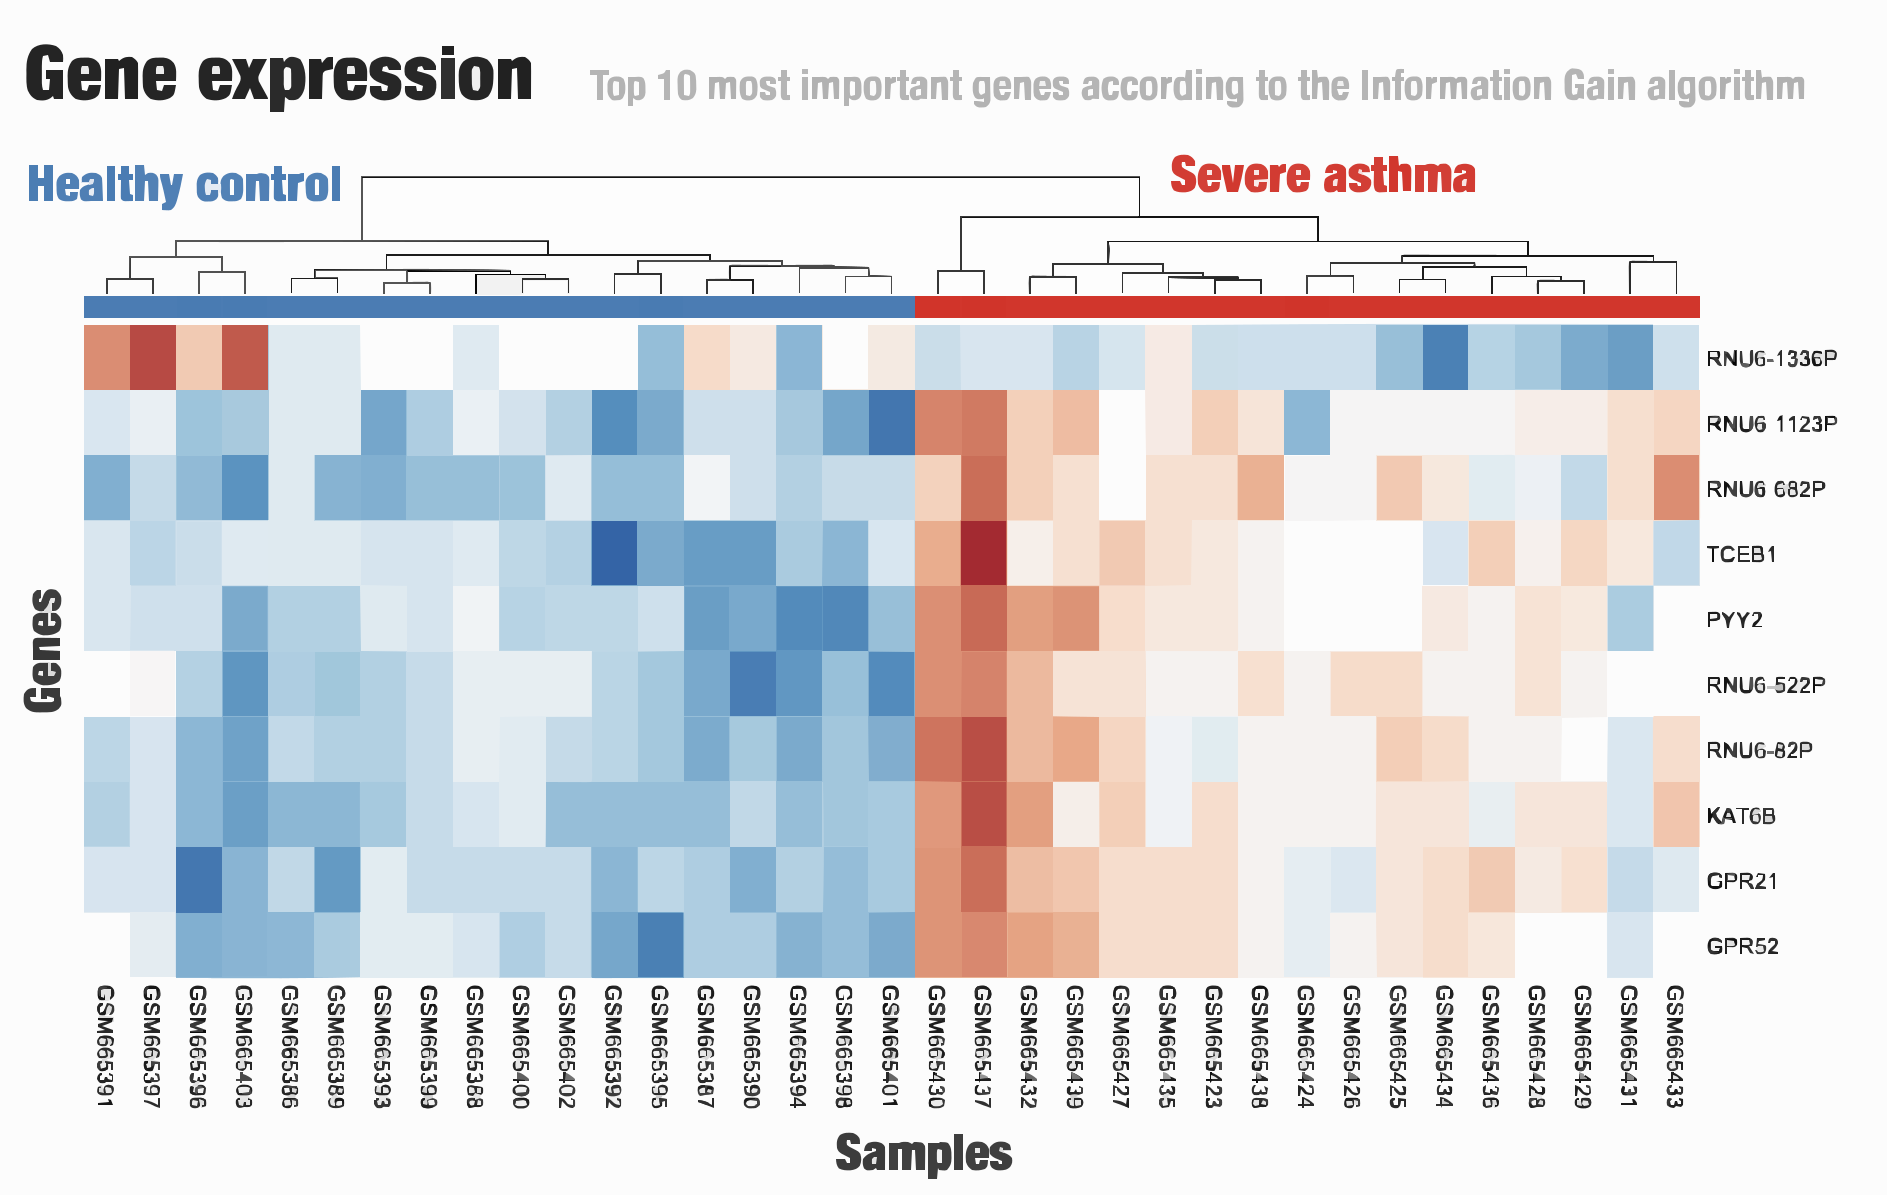
\includegraphics[width=0.8\textwidth]{figures/2-heatmap.svg}
  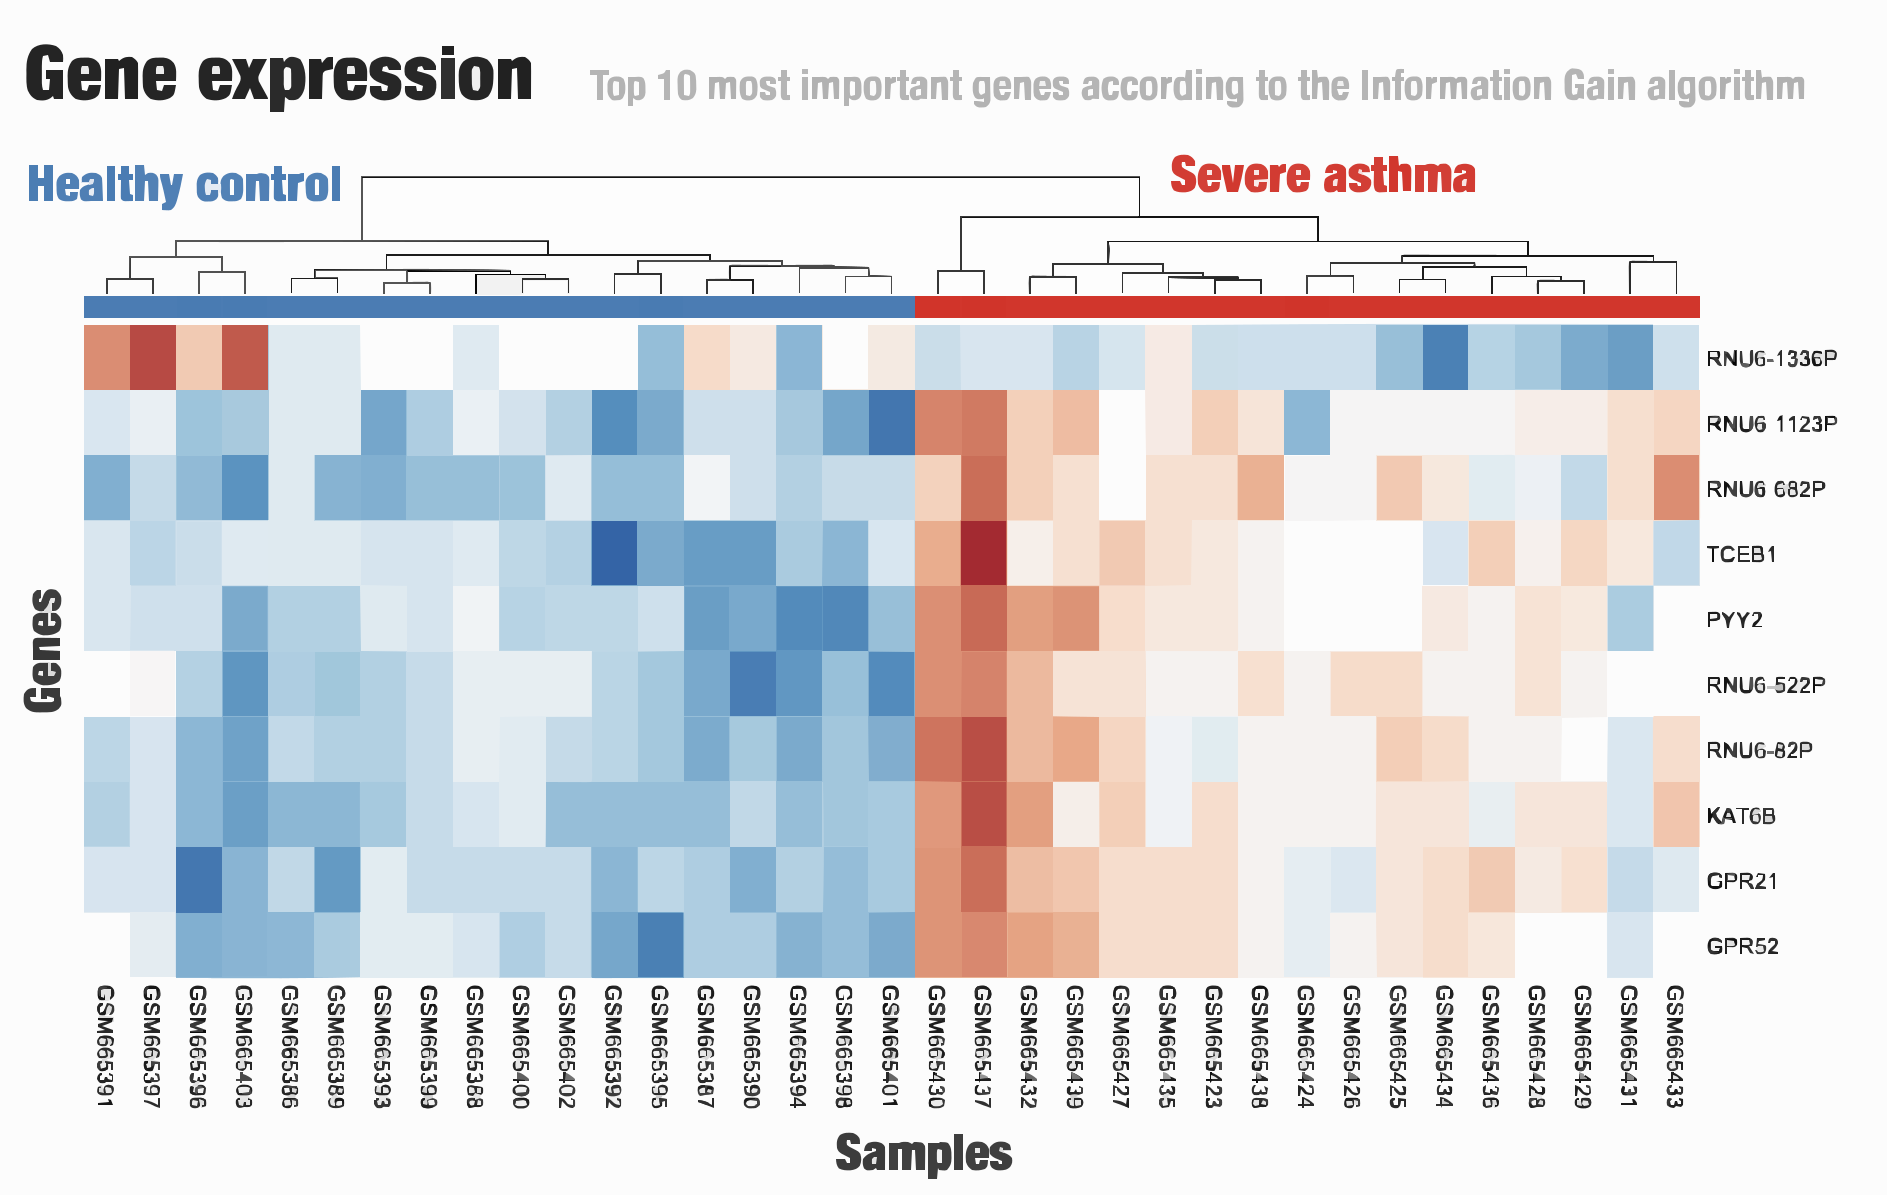
\includegraphics[width=0.8\textwidth]{figures/2-heatmap.png}
   \label{fig:2-heatmap}
  \caption{Expression levels for the top 10 most important genes by the Information Gain algorithm. Values were normalized by row. Red cells: higher gene expression levels; blue cells: lower gene expression levels. Details are available at \href{https://github.com/LBS-UFMG/asthma_microarray/blob/main/supplementary_material.pdf}{Supplementary Table S1}.}
\end{figure} % Figure 2.

\autoref{fig:2-heatmap} confirms that the genes identified by the Information Gain algorithm (\autoref{tab:3-gene-info-gain}) have expression variations consistent with their assigned class. We can observe that a group of higher-expressed genes is present in the columns for ``Severe asthma'', while less expressed genes are found in the control group section (except for \textit{RNU6-1336P}, where the opposite is true). This indicates that the genes described there may be related to asthma, but this affirmation further analysis.

Notably, \autoref{tab:3-gene-info-gain} shows small nuclear and non-coding RNA transcription genes. The importance of non-coding RNAs has been increasingly studied recently. For instance, we can cite snRNAs, which participate in pre-mRNA splicing, a process that regulates the production of protein isoforms. Our results highlight that, in diseases such as asthma, particularly in severe cases, there are alterations in gene expression that may affect the immune and inflammatory response. Therefore, it makes sense that genes linked to snRNAs stand out as essential biomarkers.

With the results provided by the Information Gain algorithm, we sought a strategy to identify genes with potential to serve as biomarkers. Hence, we used the weight distribution ($\alpha$) derived from the logistic regression model to determine the 20 genes that most positively and negatively impacted classification.

\subsection{Feature selection using Logistic Regression} % 3.4 Feature selection using Logistic Regression

The weight distribution ($\alpha$) derived from the logistic regression model indicates that most genes contribute minimally to classification, as evidenced by coefficients near zero (\autoref{fig:3-logistic-regression}A). A small subset exhibited high-magnitude weights, either positive or negative, suggesting their potential relevance for group discrimination. The ten genes with the highest and the ten genes with the lowest absolute $\alpha$ values were selected for downstream analysis (\autoref{fig:3-logistic-regression}B). Additionally, we can visually see the separation between the ``health control'' and ``severe asthma'' classes in a scatter plot of the principal components (\autoref{fig:3-logistic-regression}C).

\begin{figure}[htbp] \centering
  % 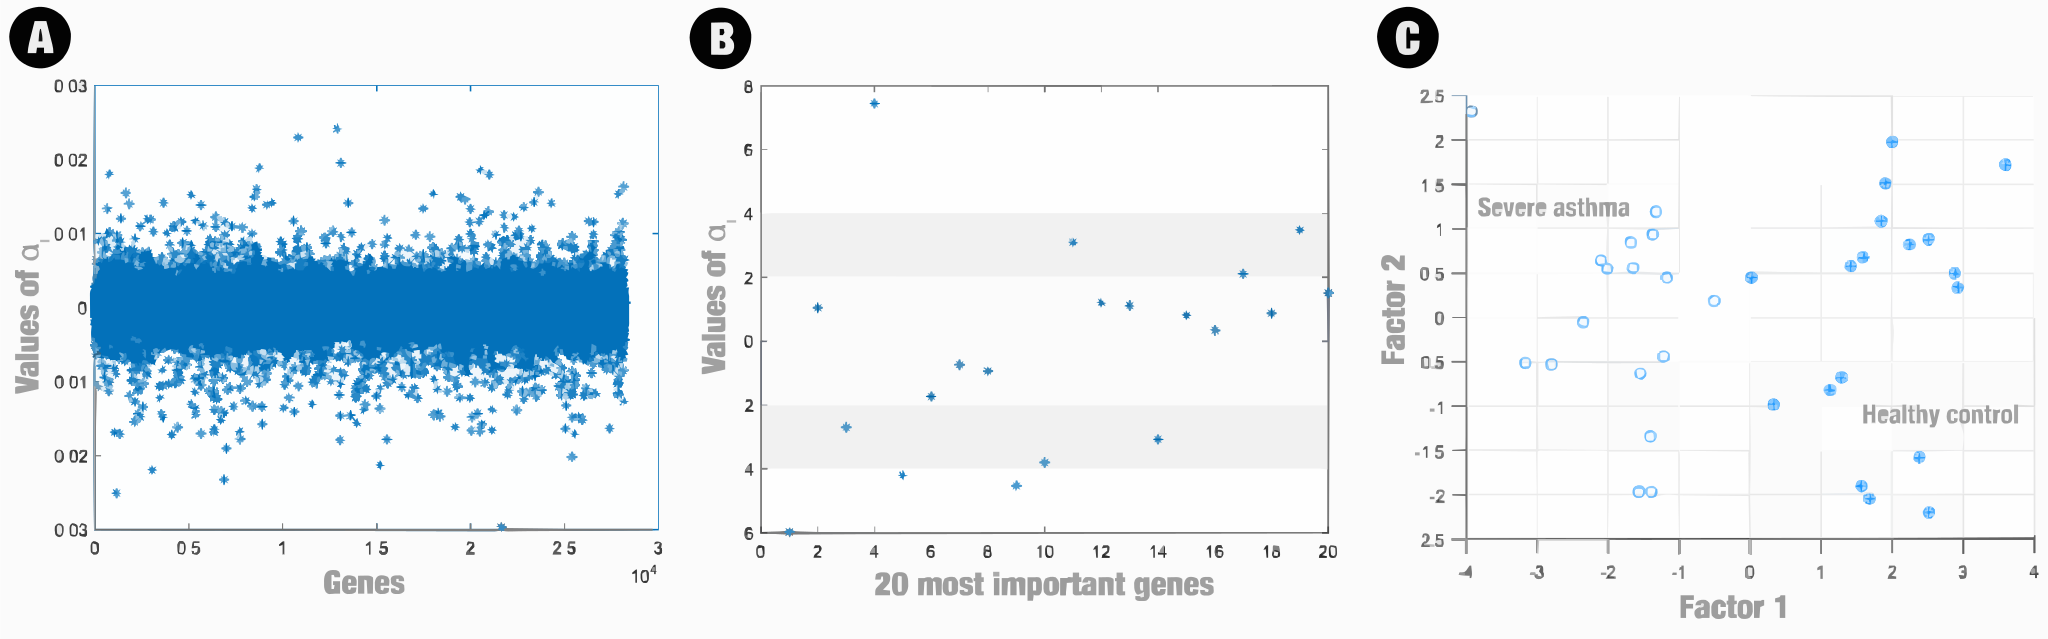
\includegraphics[width=0.8\textwidth]{figures/3-logistic_regression.svg}
  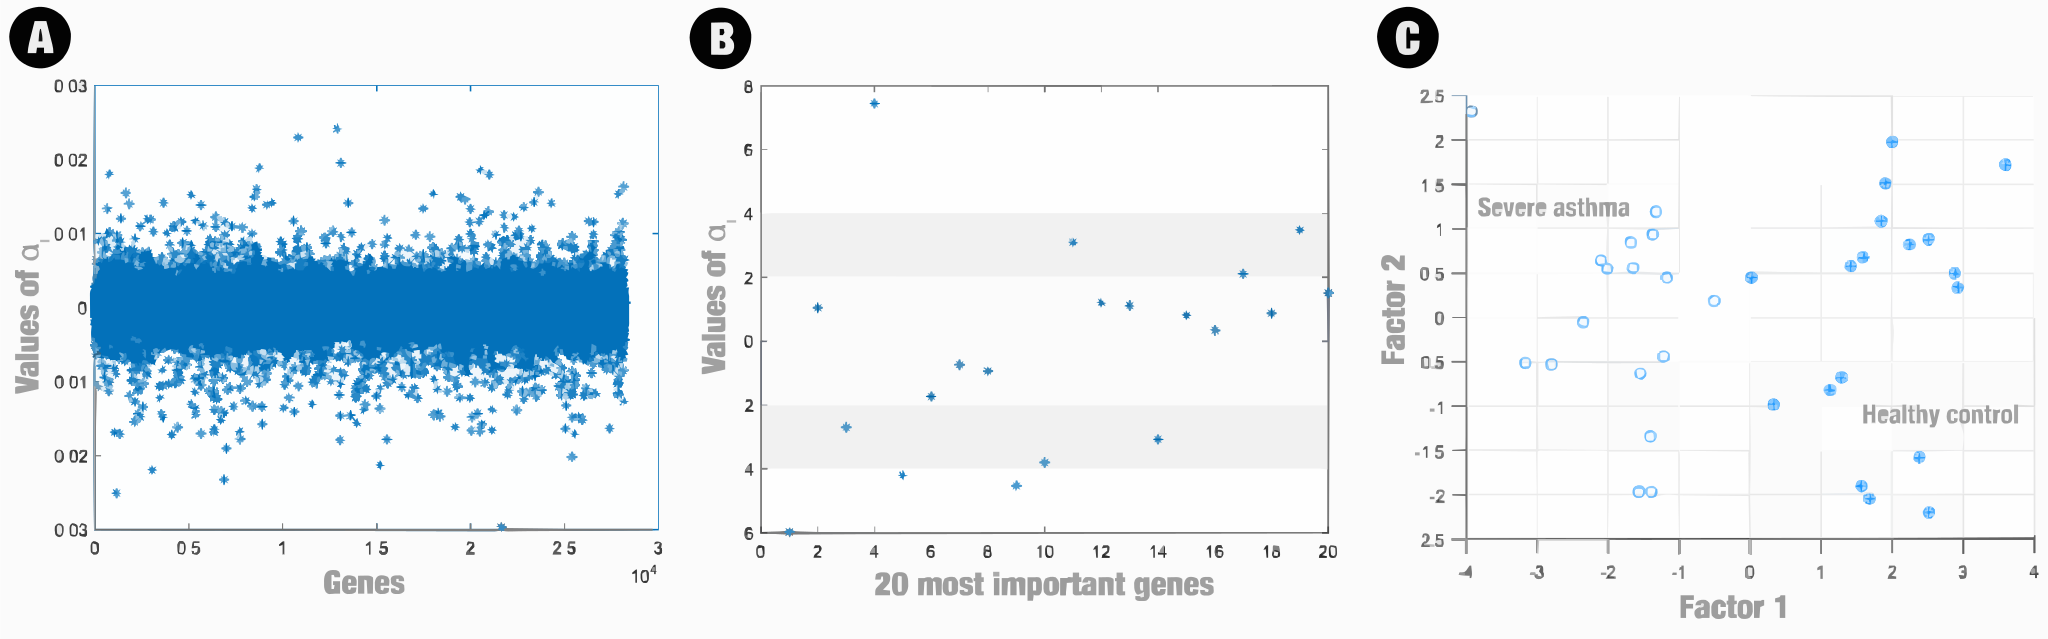
\includegraphics[width=0.8\textwidth]{figures/3-logistic_regression.png}
  \label{fig:3-logistic-regression}
  \caption{Logistic regression results. \textbf{(A)} Projection of weight distribution ($\alpha$) derived from the logistic regression model. \textbf{(B)} 20 genes that most positively (10) and negatively (10) impacted classification. \textbf{(C)} Two-dimensional representation of the projection of the 35 samples in the space. Healthy control: filled circles; severe asthma: empty circles.}
\end{figure} % Figure 3.

\autoref{tab:4-gene-logistic-importance} summarizes the main findings. Analysis of the proposed genes expression levels by the logistic regression model, show a clustering of genes that contribute positively (\href{https://github.com/LBS-UFMG/asthma_microarray/blob/main/supplementary_material.pdf}{Supplementary Figure S2}-A). However, we cannot see the same for genes that contribute negatively (\href{https://github.com/LBS-UFMG/asthma_microarray/blob/main/supplementary_material.pdf}{Supplementary Figure S2}-B).

\begin{table}[htbp] \centering
  \caption{The top 20 genes that contribute most positively (10 for Severe asthma class) and negatively (10 for Healthy controls class) to the model according to the logistic regression model}
  \label{tab:4-gene-logistic-importance}
  \begin{tabular}{cclp{4cm}clp{4cm}}
    \hline
       & \multicolumn{3}{c}{\textbf{Positive}} & \multicolumn{3}{c|}{\textbf{Negative}}                                                                                                                                                                   \\
    \hline
    \# & \textbf{Gene ID}                       & \textbf{Gene name}                     & \textbf{Description}                              & \textbf{Gene ID} & \textbf{Gene name} & \textbf{Description}                                                \\
    \hline
    1  & 8117018                                & \textit{MYLIP}                         & Myosin regulatory light chain interacting protein & 8137264          & \textit{TMEM176A}  & Transmembrane protein 176A                                          \\
    2  & 7908861                                & \textit{OCR1}                          & Ovarian cancer-related protein 1                  & 7983890          & \textit{GRINL1A}   & Myocardial zonula adherens protein                                  \\
    3  & 7967028                                & \textit{RNU4-2}                        & RNA, U4 small nuclear 2                           & 8110971          & \textit{CMBL}      & Carboxymethylenebutenolidase homolog                                \\
    4  & 7928489                                & \textit{KAT6B}                         & Lysine acetyltransferase 6B                       & 7904967          & \textit{RNVU1-19}  & Variant U1 small nuclear 19                                         \\
    5  & 8052581                                & \textit{ENSG00000278523}               & Novel ncRNA chr:2:61928634-61928704               & 8106025          & \textit{BDP1}      & Subunit of RNA polymerase III transcription initiation factor IIIB  \\
    6  & 8154211                                & \textit{JAK2}                          & Janus kinase 2                                    & 7985431          & \textit{GOLGA2P3Y} & Golgin A2 pseudogene 3, Y-linked                                    \\
    7  & 7968295                                & \textit{RNU6-82P}                      & RNA, U6 small nuclear 82, pseudogene              & 8031570          & \textit{RFPL4A}    & Ret finger protein like 4A                                          \\
    8  & 8031152                                & \textit{RPS9}                          & Ribosomal protein S9                              & 8007848          & \textit{MAPK8IP1}  & Mitogen-activated protein kinase 8 interacting protein 1 pseudogene \\
    9  & 8055639                                & \textit{ZEB2}                          & Zinc finger E-box binding homeobox 2              & 8029693          & \textit{FOSB}      & FosB proto-oncogene                                                 \\
    10 & 7975453                                & \textit{SNORD56B}                      & Small nucleolar RNA, C/D box 56B                  & 7914180          & \textit{SPCS2}     & Signal peptidase complex subunit 2                                  \\
    \hline
  \end{tabular}
\end{table} % Table 4.

Transcriptomic studies in severe asthma reveal differential expression not only of protein-coding genes, but also of non-coding RNAs, including antisense transcripts, pseudogenes and IncRNAs % [Jurkiewicz et al. 2021]
\cite{jurkiewicz_integrated_2021}. These findings highlight the potential involvement of unconventional transcripts in disease mechanisms.

Among the genes identified, \textit{JAK2} (\autoref{tab:4-gene-logistic-importance}) stands out due to its well-established for its central role in inflammatory cytokine signaling in the airways (IL-6, IL-4, IL-13) through activation of the JAK2/STAT3 pathway, targets of experimental inhibitors that have shown reductions in hyper-responsiveness and inflammation in both animal and human models % [Ren et al. 2021]
\cite{ren_zhike_2021}. The JAK2/STAT3 pathway influences asthma development by promoting inflammation and ferroptosis in airway epithelial cells. When cytokine IL-13 stimulates this pathway, it leads to the upregulation of \textit{STAT3} and \textit{JAK2} expression, which in turn increases \textit{EPAS1} expression. This activation enhances ferroptosis (a form of iron-dependent cell death) and inflammatory responses, contributing to airway damage and asthma progression. Specifically, increased JAK2/STAT3 signaling exacerbates ferroptosis and inflammation by upregulating \textit{EPAS1}, thereby amplifying airway epithelial injury associated with asthma % [Liu et al. 2025]
\cite{liu_epas1_2025}.

Other genes in \autoref{tab:4-gene-logistic-importance} exhibit more indirect or emerging associations with asthma. In a genome-wide association study (GWAS) identified an SNP (rs35514893) in the \textit{DTNBP1-MYLIP} region associated with reduced risk of exacerbations under corticosteroid therapy ($OR \approx 0.36$, $p \approx 2.9 \times 19^{-6}$), suggesting possible modulation of steroid sensitivity, though \textit{MYLIP} itself has not been directly implicated in asthma % [Hernandez-Pacheco et al. 2019]
\cite{hernandez_2019}.

Regarding non-coding RNAs, \textit{RNU4-2} which was upregulated in human bronchial epithelial cells (NHBE) after PGAP3 stimulation (log2 fold-change $\approx7.01$; $p = 0.008$), although its role in asthma is unclear % [Leslie et al. 2024]
\cite{leslie_pgap3_2024}. Similarly, \textit{SNORD56B} and \textit{RNVU1-19} have no confirmed links to asthma, despite associations with systemic inflammation or weak CNV signals, respectively % [Vishnyakova et al. 2022; Fawcett et al. 2022]
\cite{Vishnyakova_2022,fawcett_exome-wide_2022}.

In contrast, \textit{ZEB2}, a regulator of epithelial-mesenchymal transition (EMT), may influence airway remodeling. Diesel particle exposure upregulated ZEB2 in nasal epithelial cells, and its inhibition reduced polyp formation in murine models, implying a role in allergic airway inflammation % [Lee et al. 2022]
\cite{lee_2022}.

Finally, FOSB, part of the AP-1 transcription factor family, was upregulated in bronchial epithelial cells under IL-17A stimulation in severe asthma. Its expression correlated with neutrophilic inflammation and disease severity, suggesting potential involvement in inflammatory signaling, although not yet defined as a susceptibility gene % [Jakiela et al. 2023]
\cite{jakiela_bronchial_2023}. For the remaining genes, no clear associations with asthma have been documented to date.

\subsection{Limitations}

A major limitation of this work is the size of the datasets used ($n = 54$). In this study, we only used $k = 5$ cross-validation (scripts and datasets are available in the \href{https://github.com/LBS-UFMG/asthma_microarray}{supplementary material repository}). However, data obtained from microarray analyses present a special problem class, with a large number of columns ($m = 28,231$). In this context, dimensional reduction techniques, such as SVD, can represent a good solution for representing these data and removing noise. Furthermore, models based on logistic regression can handle this type of data more effectively than other machine learning algorithms, as demonstrated in our analyses (\autoref{tab:2-log-ref-mod}). This corroborates other work available in the literature % [Morais-Rodrigues et al. 2020]
\cite{morais-rodrigues_analysis_2020}. In the future, we intend to conduct additional studies to better evaluate the list of genes proposed here. Furthermore, experimental validations are necessary to confirm the results presented here.

\section{Conclusion}

This study aimed to validate previously reported asthma-associated genes and identify additional candidates with potential diagnostic or therapeutic relevance that have been little explored in the literature. Using logistic regression models, we propose a series of genes that may be related to asthma, but for which few studies are available. Our results highlight the importance of non-coding RNAs and pseudogenes. In future work, we plan to explore these results further, aiming to identify the role of these transcripts and the structural differences between genes and pseudogenes in severe asthma and healthy control groups. We hope that the results presented here can shed light on the mechanisms that lead to asthma and inform the development of new treatments.
